
% Default to the notebook output style

    


% Inherit from the specified cell style.




    
\documentclass[11pt]{article}

    
    
    \usepackage[T1]{fontenc}
    % Nicer default font (+ math font) than Computer Modern for most use cases
    \usepackage{mathpazo}

    % Basic figure setup, for now with no caption control since it's done
    % automatically by Pandoc (which extracts ![](path) syntax from Markdown).
    \usepackage{graphicx}
    % We will generate all images so they have a width \maxwidth. This means
    % that they will get their normal width if they fit onto the page, but
    % are scaled down if they would overflow the margins.
    \makeatletter
    \def\maxwidth{\ifdim\Gin@nat@width>\linewidth\linewidth
    \else\Gin@nat@width\fi}
    \makeatother
    \let\Oldincludegraphics\includegraphics
    % Set max figure width to be 80% of text width, for now hardcoded.
    \renewcommand{\includegraphics}[1]{\Oldincludegraphics[width=.8\maxwidth]{#1}}
    % Ensure that by default, figures have no caption (until we provide a
    % proper Figure object with a Caption API and a way to capture that
    % in the conversion process - todo).
    \usepackage{caption}
    \DeclareCaptionLabelFormat{nolabel}{}
    \captionsetup{labelformat=nolabel}

    \usepackage{adjustbox} % Used to constrain images to a maximum size 
    \usepackage{xcolor} % Allow colors to be defined
    \usepackage{enumerate} % Needed for markdown enumerations to work
    \usepackage{geometry} % Used to adjust the document margins
    \usepackage{amsmath} % Equations
    \usepackage{amssymb} % Equations
    \usepackage{textcomp} % defines textquotesingle
    % Hack from http://tex.stackexchange.com/a/47451/13684:
    \AtBeginDocument{%
        \def\PYZsq{\textquotesingle}% Upright quotes in Pygmentized code
    }
    \usepackage{upquote} % Upright quotes for verbatim code
    \usepackage{eurosym} % defines \euro
    \usepackage[mathletters]{ucs} % Extended unicode (utf-8) support
    \usepackage[utf8x]{inputenc} % Allow utf-8 characters in the tex document
    \usepackage{fancyvrb} % verbatim replacement that allows latex
    \usepackage{grffile} % extends the file name processing of package graphics 
                         % to support a larger range 
    % The hyperref package gives us a pdf with properly built
    % internal navigation ('pdf bookmarks' for the table of contents,
    % internal cross-reference links, web links for URLs, etc.)
    \usepackage{hyperref}
    \usepackage{longtable} % longtable support required by pandoc >1.10
    \usepackage{booktabs}  % table support for pandoc > 1.12.2
    \usepackage[inline]{enumitem} % IRkernel/repr support (it uses the enumerate* environment)
    \usepackage[normalem]{ulem} % ulem is needed to support strikethroughs (\sout)
                                % normalem makes italics be italics, not underlines
    

    
    
    % Colors for the hyperref package
    \definecolor{urlcolor}{rgb}{0,.145,.698}
    \definecolor{linkcolor}{rgb}{.71,0.21,0.01}
    \definecolor{citecolor}{rgb}{.12,.54,.11}

    % ANSI colors
    \definecolor{ansi-black}{HTML}{3E424D}
    \definecolor{ansi-black-intense}{HTML}{282C36}
    \definecolor{ansi-red}{HTML}{E75C58}
    \definecolor{ansi-red-intense}{HTML}{B22B31}
    \definecolor{ansi-green}{HTML}{00A250}
    \definecolor{ansi-green-intense}{HTML}{007427}
    \definecolor{ansi-yellow}{HTML}{DDB62B}
    \definecolor{ansi-yellow-intense}{HTML}{B27D12}
    \definecolor{ansi-blue}{HTML}{208FFB}
    \definecolor{ansi-blue-intense}{HTML}{0065CA}
    \definecolor{ansi-magenta}{HTML}{D160C4}
    \definecolor{ansi-magenta-intense}{HTML}{A03196}
    \definecolor{ansi-cyan}{HTML}{60C6C8}
    \definecolor{ansi-cyan-intense}{HTML}{258F8F}
    \definecolor{ansi-white}{HTML}{C5C1B4}
    \definecolor{ansi-white-intense}{HTML}{A1A6B2}

    % commands and environments needed by pandoc snippets
    % extracted from the output of `pandoc -s`
    \providecommand{\tightlist}{%
      \setlength{\itemsep}{0pt}\setlength{\parskip}{0pt}}
    \DefineVerbatimEnvironment{Highlighting}{Verbatim}{commandchars=\\\{\}}
    % Add ',fontsize=\small' for more characters per line
    \newenvironment{Shaded}{}{}
    \newcommand{\KeywordTok}[1]{\textcolor[rgb]{0.00,0.44,0.13}{\textbf{{#1}}}}
    \newcommand{\DataTypeTok}[1]{\textcolor[rgb]{0.56,0.13,0.00}{{#1}}}
    \newcommand{\DecValTok}[1]{\textcolor[rgb]{0.25,0.63,0.44}{{#1}}}
    \newcommand{\BaseNTok}[1]{\textcolor[rgb]{0.25,0.63,0.44}{{#1}}}
    \newcommand{\FloatTok}[1]{\textcolor[rgb]{0.25,0.63,0.44}{{#1}}}
    \newcommand{\CharTok}[1]{\textcolor[rgb]{0.25,0.44,0.63}{{#1}}}
    \newcommand{\StringTok}[1]{\textcolor[rgb]{0.25,0.44,0.63}{{#1}}}
    \newcommand{\CommentTok}[1]{\textcolor[rgb]{0.38,0.63,0.69}{\textit{{#1}}}}
    \newcommand{\OtherTok}[1]{\textcolor[rgb]{0.00,0.44,0.13}{{#1}}}
    \newcommand{\AlertTok}[1]{\textcolor[rgb]{1.00,0.00,0.00}{\textbf{{#1}}}}
    \newcommand{\FunctionTok}[1]{\textcolor[rgb]{0.02,0.16,0.49}{{#1}}}
    \newcommand{\RegionMarkerTok}[1]{{#1}}
    \newcommand{\ErrorTok}[1]{\textcolor[rgb]{1.00,0.00,0.00}{\textbf{{#1}}}}
    \newcommand{\NormalTok}[1]{{#1}}
    
    % Additional commands for more recent versions of Pandoc
    \newcommand{\ConstantTok}[1]{\textcolor[rgb]{0.53,0.00,0.00}{{#1}}}
    \newcommand{\SpecialCharTok}[1]{\textcolor[rgb]{0.25,0.44,0.63}{{#1}}}
    \newcommand{\VerbatimStringTok}[1]{\textcolor[rgb]{0.25,0.44,0.63}{{#1}}}
    \newcommand{\SpecialStringTok}[1]{\textcolor[rgb]{0.73,0.40,0.53}{{#1}}}
    \newcommand{\ImportTok}[1]{{#1}}
    \newcommand{\DocumentationTok}[1]{\textcolor[rgb]{0.73,0.13,0.13}{\textit{{#1}}}}
    \newcommand{\AnnotationTok}[1]{\textcolor[rgb]{0.38,0.63,0.69}{\textbf{\textit{{#1}}}}}
    \newcommand{\CommentVarTok}[1]{\textcolor[rgb]{0.38,0.63,0.69}{\textbf{\textit{{#1}}}}}
    \newcommand{\VariableTok}[1]{\textcolor[rgb]{0.10,0.09,0.49}{{#1}}}
    \newcommand{\ControlFlowTok}[1]{\textcolor[rgb]{0.00,0.44,0.13}{\textbf{{#1}}}}
    \newcommand{\OperatorTok}[1]{\textcolor[rgb]{0.40,0.40,0.40}{{#1}}}
    \newcommand{\BuiltInTok}[1]{{#1}}
    \newcommand{\ExtensionTok}[1]{{#1}}
    \newcommand{\PreprocessorTok}[1]{\textcolor[rgb]{0.74,0.48,0.00}{{#1}}}
    \newcommand{\AttributeTok}[1]{\textcolor[rgb]{0.49,0.56,0.16}{{#1}}}
    \newcommand{\InformationTok}[1]{\textcolor[rgb]{0.38,0.63,0.69}{\textbf{\textit{{#1}}}}}
    \newcommand{\WarningTok}[1]{\textcolor[rgb]{0.38,0.63,0.69}{\textbf{\textit{{#1}}}}}
    
    
    % Define a nice break command that doesn't care if a line doesn't already
    % exist.
    \def\br{\hspace*{\fill} \\* }
    % Math Jax compatability definitions
    \def\gt{>}
    \def\lt{<}
    % Document parameters
    \title{Chapter2 Numpy}
    
    
    

    % Pygments definitions
    
\makeatletter
\def\PY@reset{\let\PY@it=\relax \let\PY@bf=\relax%
    \let\PY@ul=\relax \let\PY@tc=\relax%
    \let\PY@bc=\relax \let\PY@ff=\relax}
\def\PY@tok#1{\csname PY@tok@#1\endcsname}
\def\PY@toks#1+{\ifx\relax#1\empty\else%
    \PY@tok{#1}\expandafter\PY@toks\fi}
\def\PY@do#1{\PY@bc{\PY@tc{\PY@ul{%
    \PY@it{\PY@bf{\PY@ff{#1}}}}}}}
\def\PY#1#2{\PY@reset\PY@toks#1+\relax+\PY@do{#2}}

\expandafter\def\csname PY@tok@w\endcsname{\def\PY@tc##1{\textcolor[rgb]{0.73,0.73,0.73}{##1}}}
\expandafter\def\csname PY@tok@c\endcsname{\let\PY@it=\textit\def\PY@tc##1{\textcolor[rgb]{0.25,0.50,0.50}{##1}}}
\expandafter\def\csname PY@tok@cp\endcsname{\def\PY@tc##1{\textcolor[rgb]{0.74,0.48,0.00}{##1}}}
\expandafter\def\csname PY@tok@k\endcsname{\let\PY@bf=\textbf\def\PY@tc##1{\textcolor[rgb]{0.00,0.50,0.00}{##1}}}
\expandafter\def\csname PY@tok@kp\endcsname{\def\PY@tc##1{\textcolor[rgb]{0.00,0.50,0.00}{##1}}}
\expandafter\def\csname PY@tok@kt\endcsname{\def\PY@tc##1{\textcolor[rgb]{0.69,0.00,0.25}{##1}}}
\expandafter\def\csname PY@tok@o\endcsname{\def\PY@tc##1{\textcolor[rgb]{0.40,0.40,0.40}{##1}}}
\expandafter\def\csname PY@tok@ow\endcsname{\let\PY@bf=\textbf\def\PY@tc##1{\textcolor[rgb]{0.67,0.13,1.00}{##1}}}
\expandafter\def\csname PY@tok@nb\endcsname{\def\PY@tc##1{\textcolor[rgb]{0.00,0.50,0.00}{##1}}}
\expandafter\def\csname PY@tok@nf\endcsname{\def\PY@tc##1{\textcolor[rgb]{0.00,0.00,1.00}{##1}}}
\expandafter\def\csname PY@tok@nc\endcsname{\let\PY@bf=\textbf\def\PY@tc##1{\textcolor[rgb]{0.00,0.00,1.00}{##1}}}
\expandafter\def\csname PY@tok@nn\endcsname{\let\PY@bf=\textbf\def\PY@tc##1{\textcolor[rgb]{0.00,0.00,1.00}{##1}}}
\expandafter\def\csname PY@tok@ne\endcsname{\let\PY@bf=\textbf\def\PY@tc##1{\textcolor[rgb]{0.82,0.25,0.23}{##1}}}
\expandafter\def\csname PY@tok@nv\endcsname{\def\PY@tc##1{\textcolor[rgb]{0.10,0.09,0.49}{##1}}}
\expandafter\def\csname PY@tok@no\endcsname{\def\PY@tc##1{\textcolor[rgb]{0.53,0.00,0.00}{##1}}}
\expandafter\def\csname PY@tok@nl\endcsname{\def\PY@tc##1{\textcolor[rgb]{0.63,0.63,0.00}{##1}}}
\expandafter\def\csname PY@tok@ni\endcsname{\let\PY@bf=\textbf\def\PY@tc##1{\textcolor[rgb]{0.60,0.60,0.60}{##1}}}
\expandafter\def\csname PY@tok@na\endcsname{\def\PY@tc##1{\textcolor[rgb]{0.49,0.56,0.16}{##1}}}
\expandafter\def\csname PY@tok@nt\endcsname{\let\PY@bf=\textbf\def\PY@tc##1{\textcolor[rgb]{0.00,0.50,0.00}{##1}}}
\expandafter\def\csname PY@tok@nd\endcsname{\def\PY@tc##1{\textcolor[rgb]{0.67,0.13,1.00}{##1}}}
\expandafter\def\csname PY@tok@s\endcsname{\def\PY@tc##1{\textcolor[rgb]{0.73,0.13,0.13}{##1}}}
\expandafter\def\csname PY@tok@sd\endcsname{\let\PY@it=\textit\def\PY@tc##1{\textcolor[rgb]{0.73,0.13,0.13}{##1}}}
\expandafter\def\csname PY@tok@si\endcsname{\let\PY@bf=\textbf\def\PY@tc##1{\textcolor[rgb]{0.73,0.40,0.53}{##1}}}
\expandafter\def\csname PY@tok@se\endcsname{\let\PY@bf=\textbf\def\PY@tc##1{\textcolor[rgb]{0.73,0.40,0.13}{##1}}}
\expandafter\def\csname PY@tok@sr\endcsname{\def\PY@tc##1{\textcolor[rgb]{0.73,0.40,0.53}{##1}}}
\expandafter\def\csname PY@tok@ss\endcsname{\def\PY@tc##1{\textcolor[rgb]{0.10,0.09,0.49}{##1}}}
\expandafter\def\csname PY@tok@sx\endcsname{\def\PY@tc##1{\textcolor[rgb]{0.00,0.50,0.00}{##1}}}
\expandafter\def\csname PY@tok@m\endcsname{\def\PY@tc##1{\textcolor[rgb]{0.40,0.40,0.40}{##1}}}
\expandafter\def\csname PY@tok@gh\endcsname{\let\PY@bf=\textbf\def\PY@tc##1{\textcolor[rgb]{0.00,0.00,0.50}{##1}}}
\expandafter\def\csname PY@tok@gu\endcsname{\let\PY@bf=\textbf\def\PY@tc##1{\textcolor[rgb]{0.50,0.00,0.50}{##1}}}
\expandafter\def\csname PY@tok@gd\endcsname{\def\PY@tc##1{\textcolor[rgb]{0.63,0.00,0.00}{##1}}}
\expandafter\def\csname PY@tok@gi\endcsname{\def\PY@tc##1{\textcolor[rgb]{0.00,0.63,0.00}{##1}}}
\expandafter\def\csname PY@tok@gr\endcsname{\def\PY@tc##1{\textcolor[rgb]{1.00,0.00,0.00}{##1}}}
\expandafter\def\csname PY@tok@ge\endcsname{\let\PY@it=\textit}
\expandafter\def\csname PY@tok@gs\endcsname{\let\PY@bf=\textbf}
\expandafter\def\csname PY@tok@gp\endcsname{\let\PY@bf=\textbf\def\PY@tc##1{\textcolor[rgb]{0.00,0.00,0.50}{##1}}}
\expandafter\def\csname PY@tok@go\endcsname{\def\PY@tc##1{\textcolor[rgb]{0.53,0.53,0.53}{##1}}}
\expandafter\def\csname PY@tok@gt\endcsname{\def\PY@tc##1{\textcolor[rgb]{0.00,0.27,0.87}{##1}}}
\expandafter\def\csname PY@tok@err\endcsname{\def\PY@bc##1{\setlength{\fboxsep}{0pt}\fcolorbox[rgb]{1.00,0.00,0.00}{1,1,1}{\strut ##1}}}
\expandafter\def\csname PY@tok@kc\endcsname{\let\PY@bf=\textbf\def\PY@tc##1{\textcolor[rgb]{0.00,0.50,0.00}{##1}}}
\expandafter\def\csname PY@tok@kd\endcsname{\let\PY@bf=\textbf\def\PY@tc##1{\textcolor[rgb]{0.00,0.50,0.00}{##1}}}
\expandafter\def\csname PY@tok@kn\endcsname{\let\PY@bf=\textbf\def\PY@tc##1{\textcolor[rgb]{0.00,0.50,0.00}{##1}}}
\expandafter\def\csname PY@tok@kr\endcsname{\let\PY@bf=\textbf\def\PY@tc##1{\textcolor[rgb]{0.00,0.50,0.00}{##1}}}
\expandafter\def\csname PY@tok@bp\endcsname{\def\PY@tc##1{\textcolor[rgb]{0.00,0.50,0.00}{##1}}}
\expandafter\def\csname PY@tok@fm\endcsname{\def\PY@tc##1{\textcolor[rgb]{0.00,0.00,1.00}{##1}}}
\expandafter\def\csname PY@tok@vc\endcsname{\def\PY@tc##1{\textcolor[rgb]{0.10,0.09,0.49}{##1}}}
\expandafter\def\csname PY@tok@vg\endcsname{\def\PY@tc##1{\textcolor[rgb]{0.10,0.09,0.49}{##1}}}
\expandafter\def\csname PY@tok@vi\endcsname{\def\PY@tc##1{\textcolor[rgb]{0.10,0.09,0.49}{##1}}}
\expandafter\def\csname PY@tok@vm\endcsname{\def\PY@tc##1{\textcolor[rgb]{0.10,0.09,0.49}{##1}}}
\expandafter\def\csname PY@tok@sa\endcsname{\def\PY@tc##1{\textcolor[rgb]{0.73,0.13,0.13}{##1}}}
\expandafter\def\csname PY@tok@sb\endcsname{\def\PY@tc##1{\textcolor[rgb]{0.73,0.13,0.13}{##1}}}
\expandafter\def\csname PY@tok@sc\endcsname{\def\PY@tc##1{\textcolor[rgb]{0.73,0.13,0.13}{##1}}}
\expandafter\def\csname PY@tok@dl\endcsname{\def\PY@tc##1{\textcolor[rgb]{0.73,0.13,0.13}{##1}}}
\expandafter\def\csname PY@tok@s2\endcsname{\def\PY@tc##1{\textcolor[rgb]{0.73,0.13,0.13}{##1}}}
\expandafter\def\csname PY@tok@sh\endcsname{\def\PY@tc##1{\textcolor[rgb]{0.73,0.13,0.13}{##1}}}
\expandafter\def\csname PY@tok@s1\endcsname{\def\PY@tc##1{\textcolor[rgb]{0.73,0.13,0.13}{##1}}}
\expandafter\def\csname PY@tok@mb\endcsname{\def\PY@tc##1{\textcolor[rgb]{0.40,0.40,0.40}{##1}}}
\expandafter\def\csname PY@tok@mf\endcsname{\def\PY@tc##1{\textcolor[rgb]{0.40,0.40,0.40}{##1}}}
\expandafter\def\csname PY@tok@mh\endcsname{\def\PY@tc##1{\textcolor[rgb]{0.40,0.40,0.40}{##1}}}
\expandafter\def\csname PY@tok@mi\endcsname{\def\PY@tc##1{\textcolor[rgb]{0.40,0.40,0.40}{##1}}}
\expandafter\def\csname PY@tok@il\endcsname{\def\PY@tc##1{\textcolor[rgb]{0.40,0.40,0.40}{##1}}}
\expandafter\def\csname PY@tok@mo\endcsname{\def\PY@tc##1{\textcolor[rgb]{0.40,0.40,0.40}{##1}}}
\expandafter\def\csname PY@tok@ch\endcsname{\let\PY@it=\textit\def\PY@tc##1{\textcolor[rgb]{0.25,0.50,0.50}{##1}}}
\expandafter\def\csname PY@tok@cm\endcsname{\let\PY@it=\textit\def\PY@tc##1{\textcolor[rgb]{0.25,0.50,0.50}{##1}}}
\expandafter\def\csname PY@tok@cpf\endcsname{\let\PY@it=\textit\def\PY@tc##1{\textcolor[rgb]{0.25,0.50,0.50}{##1}}}
\expandafter\def\csname PY@tok@c1\endcsname{\let\PY@it=\textit\def\PY@tc##1{\textcolor[rgb]{0.25,0.50,0.50}{##1}}}
\expandafter\def\csname PY@tok@cs\endcsname{\let\PY@it=\textit\def\PY@tc##1{\textcolor[rgb]{0.25,0.50,0.50}{##1}}}

\def\PYZbs{\char`\\}
\def\PYZus{\char`\_}
\def\PYZob{\char`\{}
\def\PYZcb{\char`\}}
\def\PYZca{\char`\^}
\def\PYZam{\char`\&}
\def\PYZlt{\char`\<}
\def\PYZgt{\char`\>}
\def\PYZsh{\char`\#}
\def\PYZpc{\char`\%}
\def\PYZdl{\char`\$}
\def\PYZhy{\char`\-}
\def\PYZsq{\char`\'}
\def\PYZdq{\char`\"}
\def\PYZti{\char`\~}
% for compatibility with earlier versions
\def\PYZat{@}
\def\PYZlb{[}
\def\PYZrb{]}
\makeatother


    % Exact colors from NB
    \definecolor{incolor}{rgb}{0.0, 0.0, 0.5}
    \definecolor{outcolor}{rgb}{0.545, 0.0, 0.0}



    
    % Prevent overflowing lines due to hard-to-break entities
    \sloppy 
    % Setup hyperref package
    \hypersetup{
      breaklinks=true,  % so long urls are correctly broken across lines
      colorlinks=true,
      urlcolor=urlcolor,
      linkcolor=linkcolor,
      citecolor=citecolor,
      }
    % Slightly bigger margins than the latex defaults
    
    \geometry{verbose,tmargin=1in,bmargin=1in,lmargin=1in,rmargin=1in}
    
    

    \begin{document}
    
    
    \maketitle
    
    

    
    \hypertarget{numpy-uxc18cuxac1c}{%
\section{Numpy 소개}\label{numpy-uxc18cuxac1c}}

3장과 함께 이번 장에서는 파이썬에서 인메모리 데이터를 효과적으로
적재하고 저장하고 가공하는 기법을 설명하겠다. 이 주제는 매우 광범위하다.
데이터세트는 광범위한 원천으로부터 문서나 이미지, 사운드 클립, 수치
측정값 등 거의 모든 것을 아우르는 매우 다양한 형식으로 들어올 수 있다.
이렇게 명백한 다양성에도 불구하고 모든 데이터를 근본적으로 숫자 배열로
간주하는 것이 도움이 될 것이다.

예를 들어, 이미지(특히, 디지털 이미지)는 단순히 해당 영역에 대한 픽셀
밝기를 나타내는 2차원 숫자 배열로 생각할 수 있다. 사운드 클립은 시간
대비 강도(intensity)를 나타내는 일차원 배열로 생각할 수 있다. 텍스트는
특정 단어나 단어 쌍의 빈도를 나타내는 이진수처럼 다양한 방식을 통해
수치로 전환할 수 있다. 데이터가 무엇이든 상관없이 그 데이터를 분석할 수
있게 만드는 첫 번째 단계는 데이터를 숫자 배열로 변환하는 것이다. (이
절차에 대한 몇 가지 예제를 429쪽 '특징 공학'에서 살펴본다.) 이러한
이유로 숫자 배열을 효과적으로 저장하고 가공하는 것은 데이터 과학을
수행하는 절차에서 가장 근본적인 작업이다. 잊 ㅔ파이썬이 이러한 숫자
배열을 다루기 위해 제공하는 전문 도구인 NumPy 패키지와 Pandas
패키지(3장)를 살펴보겠다. 이번 장에서는 NumPy에 대해 자세히 다룬다.
NumPy(Numerical Python의 약자)는 조밀한 데이터 버퍼에서 저장하고
처리하는 효과적인 인터페이스를 제공한다. 어떤 면에서 보면 NumPy 배열은
파이썬 내장 타입인 list와 비슷하지만 배열의 규모가 커질수록 데이터 저장
및 처리에 훨씬 더 효율적이다. NumPy 배열은 파이썬의 데이터 과학 도구로
구성된 전체 생태계의 핵심을 이루고 있기 때문에 관심 있는 데이터 과학
측면이 무엇이든 상관없이 NumPy를 효과적으로 사용하는 법을 배워야 한다.
서문에서 권고했던 내용에 따라 아나콘다 스택을 설치했다면 이미 NumPy가
설치돼 있을 것이다. 뭐든 직접 해 보기를 좋아한느 독자라면 NumPy
웹사이트에 가서 설치 안내에 따라 설치하면 된다. 설치하고 나면 NumPy를
임포트하고 버전을 재확인할 수 있다.

    \begin{Verbatim}[commandchars=\\\{\}]
{\color{incolor}In [{\color{incolor}1}]:} \PY{k+kn}{import} \PY{n+nn}{numpy}
        \PY{n}{numpy}\PY{o}{.}\PY{n}{\PYZus{}\PYZus{}version\PYZus{}\PYZus{}}
\end{Verbatim}


\begin{Verbatim}[commandchars=\\\{\}]
{\color{outcolor}Out[{\color{outcolor}1}]:} '1.15.1'
\end{Verbatim}
            
    이 책에서는 NumPy 버전 1.8 이상을 추천한다. 관례상 SciPy와 PyData를
사용하는 대부분의 사용자는 NumPy를 별칭(alias)인 np를 사용해 임포트한다.

    \begin{Verbatim}[commandchars=\\\{\}]
{\color{incolor}In [{\color{incolor}2}]:} \PY{k+kn}{import} \PY{n+nn}{numpy} \PY{k}{as} \PY{n+nn}{np}
\end{Verbatim}


    이번 장을 비롯한 이 책의 나머지 부분에서도 이처럼 NumPy를 임포트하고
사용하는 것을 보게 될 것이다.

\hypertarget{uxb0cauxb0b4uxc7a5-uxbb38uxc11cuxac00-uxc788uxc74cuxc744-uxae30uxc5b5uxd558uxc790}{%
\subsubsection{냊내장 문서가 있음을
기억하자!}\label{uxb0cauxb0b4uxc7a5-uxbb38uxc11cuxac00-uxc788uxc74cuxc744-uxae30uxc5b5uxd558uxc790}}

이번 장을 읽을 때 IPython에서는 탭 자동 완성 기능을 사용해 패키지의
내용을 빠르게 탐색할 수 있고 ? 기호를 사용해 다양한 함수의 문서를 확인할
수 있다는 사실을 잊지 말자. 이 기능이 잘 기억나지 않는다면 3쪽'IPython의
도움말과 문서'를 참고하라

예를 들어, numpy 네임스페이스의 모든 내용을 표시하고 싶담녀 다음과 같이
입력하면 된다. np. NumPy의 내장 문서를 표시하려면 다음 명령어를 사용하면
된다. np? 튜토리얼과 다른 참고자료와 함께 더 자세한 문서는 넘파이
홈페이지 에서 확인할 수 있다.

    \hypertarget{uxd30cuxc774uxc36cuxc758-uxb370uxc774uxd130-uxd0c0uxc785-uxc774uxd574uxd558uxae30}{%
\subsection{파이썬의 데이터 타입
이해하기}\label{uxd30cuxc774uxc36cuxc758-uxb370uxc774uxd130-uxd0c0uxc785-uxc774uxd574uxd558uxae30}}

효과적인 데이터 기반 과학 및 계산을 위해서는 데이터가 어떻게 저장되고
가공되는지 이해해야 한다. 이번 절에서는 데이터 배열이 파이썬 언어
자체에서 어떻게 처리되는지 간단히 설명하고 비교한 뒤, NumPy가 이를
어떻게 개선하는지 알아볼 것이다. 이 차이점을 이해하는 것은 책 나머지에
등장하는 많은 자료를 이해하는데 기초가 될 것이다. 파이썬 사용자는 대채로
파이썬의 사용 편의성에 끌리는데 그중 하나가 동적 타이핑이다. C나 자바
같은 정적 타입 체계를 가진 언어는 모든 변수를 명시적으로 선언해야
하지만, 파이썬처럼 동적 타입 체계를 가진 언어는 타입을 지정하지 않아도
된다. 예를 들어, C에서는 특정 연산을 다음과 같이 지정할 것이다.

    \begin{Verbatim}[commandchars=\\\{\}]
{\color{incolor}In [{\color{incolor}3}]:} \PY{c+c1}{\PYZsh{} int result=0;}
        \PY{c+c1}{\PYZsh{} for(int i=0; i\PYZlt{} 100; i++)\PYZob{}}
        \PY{c+c1}{\PYZsh{}     result += i;}
        \PY{c+c1}{\PYZsh{} \PYZcb{}}
\end{Verbatim}


    \begin{Verbatim}[commandchars=\\\{\}]
{\color{incolor}In [{\color{incolor}4}]:} \PY{n}{result} \PY{o}{=} \PY{l+m+mi}{0}
        \PY{k}{for} \PY{n}{i} \PY{o+ow}{in} \PY{n+nb}{range}\PY{p}{(}\PY{l+m+mi}{100}\PY{p}{)}\PY{p}{:}
            \PY{n}{result} \PY{o}{+}\PY{o}{=} \PY{n}{i}
\end{Verbatim}


    주요 차이점을 알겠는가? C에서는 각 변수의 데이터 타입을 명시적으로
선언했지만, 파이썬은 타입을 동적으로 추론한다. 이것은 곧 모든 변수에
어떤 종류의 데이터든 할당할 수 있다는 뜻이다.

    \begin{Verbatim}[commandchars=\\\{\}]
{\color{incolor}In [{\color{incolor}5}]:} \PY{n}{x} \PY{o}{=} \PY{l+m+mi}{4}
        \PY{n}{x} \PY{o}{=} \PY{l+s+s2}{\PYZdq{}}\PY{l+s+s2}{four}\PY{l+s+s2}{\PYZdq{}}
\end{Verbatim}


    위 코드는 x의 내용을 정수에서 문자열로 바꾼 것이다. C에서 똑같이 작업을
하면 컴파일러 에러나 다른 의도하지 않은 결과가 발생할 수도 있다. 이러한
유연성은 파이썬과 다른 동적 타입 지정 언어를 사용하기 편하고 쉽게 만드는
특징 중 하나다. 이것이 어떻게 가능한지를 이해하는 것이 파이썬으로
효과적으로 효율적으로 데이터를 분석하는 법을 배우는데 중요한 부분이다.
그러나 이러한 유연성은 또한 파이썬 변수가 그 값 이상의 무언가를
나타낸다는 뜻이기도 하다. 즉, 변수는 그 값의 유형에 대한 부가 정보도
함께 담고 있다. 다음 절에서 이에 대해 더 자세히 살펴보자.

    \hypertarget{uxd30cuxc774uxc36c-uxc815uxc218uxb294-uxc815uxc218-uxc774uxc0c1uxc774uxb2e4}{%
\paragraph{파이썬 정수는 정수
이상이다}\label{uxd30cuxc774uxc36c-uxc815uxc218uxb294-uxc815uxc218-uxc774uxc0c1uxc774uxb2e4}}

표준 파이썬은 C로 구현돼 잇다. 이 말은 곧 모든 파이썬 객체가 그 값뿐만
아니라 다른 정보까지 포함하는 똑똑하게 위장한 C 구조체라는 뜻이다. 예를
들어, x = 10000과 같이 파이썬에서 정수를 정의할 때 x는 단순히 있는
그대로의 정수를 의미하지 않는다. 실제로는 여러 값이 들어 있는 복합적인 C
구조체다. C 매크로를 확장하여 파이썬 3.6 소스코드를 보면 정수(long)타입
정의가 실제로 다음과 같이 돼있다.

\begin{verbatim}
struct _longobject{
    long ob_refcnt;
    PyTypeObject *ob_type;
    size_t ob_size;
    long ob_digit[1];
};
\end{verbatim}

파이썬 3.6의 단일 정수는 실제로 다음 네 가지 구성요소를 갖는다.

\begin{itemize}
\tightlist
\item
  ob\_refcnt: 파이썬이 조용히 메모리 할당과 해제를 처리할 수 있게 돕는
  참조 횟수
\item
  ob\_type: 변수 타입을 인코딩
\item
  ob\_size: 다음 데이터 멤버의 크기를 지정
\item
  ob\_digit: 파이썬 변수가 나타내는 실제 정숫값을 포함
  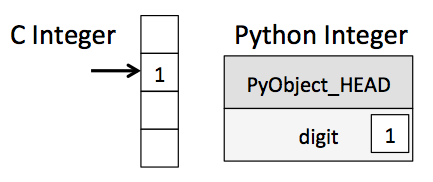
\includegraphics{cint_vs_pyint.png}
\end{itemize}

이것은 그림 2-1처럼 C와 같은 컴파일 언어에서 정수를 저장하는 것에 비해
파이썬에서 정수를 저장할때 어느정도 오버헤드가 있다는 의미다. 여기서
PyObject\_Head는 참조 횟수, 타입 코드, 그리고 전에 언급한 다른 정보를
포함한 구조체의 일부다. 차이점이라면 C 정수는 근본적으로 정숫값을
나타내는 바이트를 포함하는 메모리 위치를 가리키는 레이블이고 파이썬
정수는 정숫값을 담고 있는 바이트를 포함한 모든 파이썬 객체 정보를
포함하는 메모리의 위치를 가리키는 포인터라는 사실이다. 파이썬 정수
구조체의 이 추가 정보 덕분에 파이썬에서 그토록 자유롭게 동적을 코드를
작설할 수 있는 것이다. 하지만 파이썬 타입에 있는 모든 추가 정보에는
비용이 따르며, 특히 이 객체들을 여러 개 결합하는 구조에서 그 비용이
분명하게 드러난다.

    \hypertarget{uxd30cuxc774uxc36c-uxb9acuxc2a4uxd2b8uxb294-uxb9acuxc2a4uxd2b8-uxc774uxc0c1uxc774uxb2e4}{%
\paragraph{파이썬 리스트는 리스트
이상이다}\label{uxd30cuxc774uxc36c-uxb9acuxc2a4uxd2b8uxb294-uxb9acuxc2a4uxd2b8-uxc774uxc0c1uxc774uxb2e4}}

이번에는 여러 개의 파이썬 객체를 담은 파이썬 자료 구조를 사용할 때 어떤
일이 벌어지는지 생각해 보자. 파이썬에서 여러 개의 요소를 담는 가변적인
표준 컨테이너는 리스트다. 다음과 같이 정수 리스트를 만들 수 있다.

    \begin{Verbatim}[commandchars=\\\{\}]
{\color{incolor}In [{\color{incolor}6}]:} \PY{n}{L} \PY{o}{=} \PY{n+nb}{list}\PY{p}{(}\PY{n+nb}{range}\PY{p}{(}\PY{l+m+mi}{10}\PY{p}{)}\PY{p}{)}
        \PY{n}{L}
\end{Verbatim}


\begin{Verbatim}[commandchars=\\\{\}]
{\color{outcolor}Out[{\color{outcolor}6}]:} [0, 1, 2, 3, 4, 5, 6, 7, 8, 9]
\end{Verbatim}
            
    \begin{Verbatim}[commandchars=\\\{\}]
{\color{incolor}In [{\color{incolor}7}]:} \PY{n+nb}{type}\PY{p}{(}\PY{n}{L}\PY{p}{[}\PY{l+m+mi}{0}\PY{p}{]}\PY{p}{)}
\end{Verbatim}


\begin{Verbatim}[commandchars=\\\{\}]
{\color{outcolor}Out[{\color{outcolor}7}]:} int
\end{Verbatim}
            
    \begin{Verbatim}[commandchars=\\\{\}]
{\color{incolor}In [{\color{incolor}8}]:} \PY{n}{L2} \PY{o}{=} \PY{p}{[}\PY{n+nb}{str}\PY{p}{(}\PY{n}{c}\PY{p}{)} \PY{k}{for} \PY{n}{c} \PY{o+ow}{in} \PY{n}{L}\PY{p}{]}
        \PY{n}{L2}
\end{Verbatim}


\begin{Verbatim}[commandchars=\\\{\}]
{\color{outcolor}Out[{\color{outcolor}8}]:} ['0', '1', '2', '3', '4', '5', '6', '7', '8', '9']
\end{Verbatim}
            
    \begin{Verbatim}[commandchars=\\\{\}]
{\color{incolor}In [{\color{incolor}9}]:} \PY{n+nb}{type}\PY{p}{(}\PY{n}{L2}\PY{p}{[}\PY{l+m+mi}{0}\PY{p}{]}\PY{p}{)}
\end{Verbatim}


\begin{Verbatim}[commandchars=\\\{\}]
{\color{outcolor}Out[{\color{outcolor}9}]:} str
\end{Verbatim}
            
    파이썬의 동적 타이핑(dynamic typing) 덕북에 서로 다른 데이터 타입의
요소를 담는 리스트를 만들 수도 있다.

    \begin{Verbatim}[commandchars=\\\{\}]
{\color{incolor}In [{\color{incolor}10}]:} \PY{n}{L3} \PY{o}{=} \PY{p}{[}\PY{k+kc}{True}\PY{p}{,} \PY{l+s+s2}{\PYZdq{}}\PY{l+s+s2}{2}\PY{l+s+s2}{\PYZdq{}}\PY{p}{,} \PY{l+m+mf}{3.0}\PY{p}{,} \PY{l+m+mi}{4}\PY{p}{]}
         \PY{p}{[}\PY{n+nb}{type}\PY{p}{(}\PY{n}{item}\PY{p}{)} \PY{k}{for} \PY{n}{item} \PY{o+ow}{in} \PY{n}{L3}\PY{p}{]}
\end{Verbatim}


\begin{Verbatim}[commandchars=\\\{\}]
{\color{outcolor}Out[{\color{outcolor}10}]:} [bool, str, float, int]
\end{Verbatim}
            
    그러나 이 유연성에는 비용이 따른다. 이렇게 유연한 타입을 허용하려면
리스트의 각 항목에 타입 정보와 참조 횟수, 기타 정보가 들어가야 한다. 즉,
각 항목이 완전한 파이썬 객체인 셈이다. 모든 변수가 같은 타입인 경우에는
이 정보가 대부분 불필요하게 중복되므로 고정 타입 배열에 데이터를
저장하는 것이 더 효율적일 수 있다. 동적 타입 리스트와 고정 타입(NumPy
스타일) 배열의 차이는 그림 2-2에 그림 으로 나타냈다. 구현 레벨에서는
배열이 근본적으로 인접한 데이터 블록을 가리키는 단일 포인터를 담고 있다.
반면 파이썬 리스트는 앞에서 본 파이썬 정수와 같이 완전한 파이썬 객체를
차례로 가리키는 포인터의 블록을 가리키는 포인터를 담고 있다. 다시
말하지만, 리스트의 장점은 유연성이다. 각 리스트 요소가 데이터와 타입
정보를 포함하는 완전한 구조이기 때문에 리스트를 어떤 타입으로도 채울 수
있다. 고정 타입의 NumPy 스타일 배열은 이러한 유연성은 부족하지만
데이터를 저장하고 가공하기에는 훨씬 더 효율적이다.

\includegraphics{attachment:image.png}- 이미지 추가

\hypertarget{uxd30cuxc774uxc36cuxc758-uxace0uxc815-uxd0c0uxc785-uxbc30uxc5f4}{%
\paragraph{파이썬의 고정 타입
배열}\label{uxd30cuxc774uxc36cuxc758-uxace0uxc815-uxd0c0uxc785-uxbc30uxc5f4}}

파이썬은 데이터를 효율적인 고정 타입 데이터 버퍼에 저장하는 다양한
방식을 제공한다. 내장 array 모듈은 단일 조합의 조밀한 배열(dense
array)을 만드는 데 사용할 수 잇다.

    \begin{Verbatim}[commandchars=\\\{\}]
{\color{incolor}In [{\color{incolor}11}]:} \PY{k+kn}{import} \PY{n+nn}{array}
         \PY{n}{L} \PY{o}{=}\PY{n+nb}{list}\PY{p}{(}\PY{n+nb}{range}\PY{p}{(}\PY{l+m+mi}{10}\PY{p}{)}\PY{p}{)}
         \PY{n}{A} \PY{o}{=}\PY{n}{array}\PY{o}{.}\PY{n}{array}\PY{p}{(}\PY{l+s+s1}{\PYZsq{}}\PY{l+s+s1}{i}\PY{l+s+s1}{\PYZsq{}}\PY{p}{,} \PY{n}{L}\PY{p}{)}
         \PY{n}{A}
\end{Verbatim}


\begin{Verbatim}[commandchars=\\\{\}]
{\color{outcolor}Out[{\color{outcolor}11}]:} array('i', [0, 1, 2, 3, 4, 5, 6, 7, 8, 9])
\end{Verbatim}
            
    여기서 'i'는 내용이 정수임을 가리키는 타입 코드다. 그러나 훨씬 더 유용한
것은 NumPy 패키지의 ndarray 객체다. 파이썬의 array 객첸느 배열 기반의
데이터에 효율적인 저장소를 제공한느 반면, NumPy는 그 데이터에 효율적인
연산을 추갛나다. 이러한 연산에 대해서는 뒤에서 알아보고 여기서는 NumPy
배열을 생성하는 여러 방법을 살펴보자. 먼저 별칭 np로 표준 NumPy를
임포트하자.

    \begin{Verbatim}[commandchars=\\\{\}]
{\color{incolor}In [{\color{incolor}12}]:} \PY{k+kn}{import} \PY{n+nn}{numpy} \PY{k}{as} \PY{n+nn}{np}
\end{Verbatim}


    \hypertarget{uxd30cuxc774uxc36c-uxb9acuxc2a4uxd2b8uxc5d0uxc11c-uxbc30uxc5f4-uxb9ccuxb4e4uxae30}{%
\paragraph{파이썬 리스트에서 배열
만들기}\label{uxd30cuxc774uxc36c-uxb9acuxc2a4uxd2b8uxc5d0uxc11c-uxbc30uxc5f4-uxb9ccuxb4e4uxae30}}

우선 np.array를 사용해 파이썬 리스트에서 배열을 만들 수 있다.

    \begin{Verbatim}[commandchars=\\\{\}]
{\color{incolor}In [{\color{incolor}13}]:} \PY{c+c1}{\PYZsh{}정수 배열}
         \PY{n}{np}\PY{o}{.}\PY{n}{array}\PY{p}{(}\PY{p}{[}\PY{l+m+mi}{1}\PY{p}{,} \PY{l+m+mi}{4}\PY{p}{,} \PY{l+m+mi}{2}\PY{p}{,} \PY{l+m+mi}{5}\PY{p}{,} \PY{l+m+mi}{3}\PY{p}{]}\PY{p}{)}
\end{Verbatim}


\begin{Verbatim}[commandchars=\\\{\}]
{\color{outcolor}Out[{\color{outcolor}13}]:} array([1, 4, 2, 5, 3])
\end{Verbatim}
            
    파이썬의 리스트와 달리 NumPy는 배열의 모든 요소가 같은 타입이어야 한다는
점을 기억하라. 타입이 일치하지 않으면 NumPy는 가능한 경우 상위 타입을
취하게 된다.(다음에서 정수는 상위 타입인 부동 소수점으로 변환된다)

    \begin{Verbatim}[commandchars=\\\{\}]
{\color{incolor}In [{\color{incolor}14}]:} \PY{n}{np}\PY{o}{.}\PY{n}{array}\PY{p}{(}\PY{p}{[}\PY{l+m+mf}{3.14}\PY{p}{,} \PY{l+m+mi}{4}\PY{p}{,} \PY{l+m+mi}{2}\PY{p}{,} \PY{l+m+mi}{3}\PY{p}{]}\PY{p}{)}
\end{Verbatim}


\begin{Verbatim}[commandchars=\\\{\}]
{\color{outcolor}Out[{\color{outcolor}14}]:} array([3.14, 4.  , 2.  , 3.  ])
\end{Verbatim}
            
    명시적인 결과 배열의 데이터 타입을 설정하려면 dtype 키워드를 사용하면
된다.

    \begin{Verbatim}[commandchars=\\\{\}]
{\color{incolor}In [{\color{incolor}15}]:} \PY{n}{np}\PY{o}{.}\PY{n}{array}\PY{p}{(}\PY{p}{[}\PY{l+m+mi}{1}\PY{p}{,} \PY{l+m+mi}{2}\PY{p}{,} \PY{l+m+mi}{3}\PY{p}{,} \PY{l+m+mi}{4}\PY{p}{]}\PY{p}{,} \PY{n}{dtype}\PY{o}{=}\PY{l+s+s1}{\PYZsq{}}\PY{l+s+s1}{float32}\PY{l+s+s1}{\PYZsq{}}\PY{p}{)}
\end{Verbatim}


\begin{Verbatim}[commandchars=\\\{\}]
{\color{outcolor}Out[{\color{outcolor}15}]:} array([1., 2., 3., 4.], dtype=float32)
\end{Verbatim}
            
    마지막으로 파이썬 리스트와는 달리 NumPy 배열은 명시적으로 다차원이
가능하다. 다음은 리스트의 리스트를 사용해 다차원 배열을 초기화하는 한
가지 방법이다.

    \begin{Verbatim}[commandchars=\\\{\}]
{\color{incolor}In [{\color{incolor}16}]:} \PY{c+c1}{\PYZsh{}리스트를 중첩하면 다차원 배열이 됨}
         \PY{n}{np}\PY{o}{.}\PY{n}{array}\PY{p}{(}\PY{p}{[}\PY{n+nb}{range}\PY{p}{(}\PY{n}{i}\PY{p}{,} \PY{n}{i}\PY{o}{+}\PY{l+m+mi}{3}\PY{p}{)} \PY{k}{for} \PY{n}{i} \PY{o+ow}{in} \PY{p}{[}\PY{l+m+mi}{2}\PY{p}{,} \PY{l+m+mi}{4}\PY{p}{,} \PY{l+m+mi}{6}\PY{p}{]}\PY{p}{]}\PY{p}{)}
\end{Verbatim}


\begin{Verbatim}[commandchars=\\\{\}]
{\color{outcolor}Out[{\color{outcolor}16}]:} array([[2, 3, 4],
                [4, 5, 6],
                [6, 7, 8]])
\end{Verbatim}
            
    내부 리스트는 결과로 얻은 이차원 배열의 행으로 취급된다.

    \hypertarget{uxcc98uxc74cuxbd80uxd130-uxbc30uxc5f4-uxb9ccuxb4e4uxae30}{%
\paragraph{처음부터 배열
만들기}\label{uxcc98uxc74cuxbd80uxd130-uxbc30uxc5f4-uxb9ccuxb4e4uxae30}}

특히 규모가 큰 배열의 경우에는 NumPy에 내장된 루틴을 사용해 처음부터
배열을 생성하는 것이 더 효율적이다.

    \begin{Verbatim}[commandchars=\\\{\}]
{\color{incolor}In [{\color{incolor}17}]:} \PY{c+c1}{\PYZsh{} 0으로 채운 길이 10의 정수 배열 만들기}
         \PY{n}{np}\PY{o}{.}\PY{n}{zeros}\PY{p}{(}\PY{l+m+mi}{10}\PY{p}{,} \PY{n}{dtype}\PY{o}{=}\PY{n+nb}{int}\PY{p}{)}
\end{Verbatim}


\begin{Verbatim}[commandchars=\\\{\}]
{\color{outcolor}Out[{\color{outcolor}17}]:} array([0, 0, 0, 0, 0, 0, 0, 0, 0, 0])
\end{Verbatim}
            
    \begin{Verbatim}[commandchars=\\\{\}]
{\color{incolor}In [{\color{incolor}18}]:} \PY{c+c1}{\PYZsh{} 1로 채운 3x5 부동 소수점 배열 만들기}
         \PY{n}{np}\PY{o}{.}\PY{n}{ones}\PY{p}{(}\PY{p}{(}\PY{l+m+mi}{3}\PY{p}{,} \PY{l+m+mi}{5}\PY{p}{)}\PY{p}{,} \PY{n}{dtype}\PY{o}{=}\PY{n+nb}{float}\PY{p}{)}
\end{Verbatim}


\begin{Verbatim}[commandchars=\\\{\}]
{\color{outcolor}Out[{\color{outcolor}18}]:} array([[1., 1., 1., 1., 1.],
                [1., 1., 1., 1., 1.],
                [1., 1., 1., 1., 1.]])
\end{Verbatim}
            
    \begin{Verbatim}[commandchars=\\\{\}]
{\color{incolor}In [{\color{incolor}19}]:} \PY{c+c1}{\PYZsh{} 3.14로 채운 3x5 배열 만들기}
         \PY{n}{np}\PY{o}{.}\PY{n}{full}\PY{p}{(}\PY{p}{(}\PY{l+m+mi}{3}\PY{p}{,} \PY{l+m+mi}{5}\PY{p}{)}\PY{p}{,} \PY{l+m+mf}{3.14}\PY{p}{)}
\end{Verbatim}


\begin{Verbatim}[commandchars=\\\{\}]
{\color{outcolor}Out[{\color{outcolor}19}]:} array([[3.14, 3.14, 3.14, 3.14, 3.14],
                [3.14, 3.14, 3.14, 3.14, 3.14],
                [3.14, 3.14, 3.14, 3.14, 3.14]])
\end{Verbatim}
            
    \begin{Verbatim}[commandchars=\\\{\}]
{\color{incolor}In [{\color{incolor}20}]:} \PY{c+c1}{\PYZsh{}선형 수열로 채운 3x5 배열 만들기}
         \PY{c+c1}{\PYZsh{} 0에서 시작해 2식 더해 20까지 채움}
         \PY{c+c1}{\PYZsh{} 내장 함수인 range()와 유사}
         \PY{n}{np}\PY{o}{.}\PY{n}{arange}\PY{p}{(}\PY{l+m+mi}{0}\PY{p}{,} \PY{l+m+mi}{20}\PY{p}{,} \PY{l+m+mi}{2}\PY{p}{)}
\end{Verbatim}


\begin{Verbatim}[commandchars=\\\{\}]
{\color{outcolor}Out[{\color{outcolor}20}]:} array([ 0,  2,  4,  6,  8, 10, 12, 14, 16, 18])
\end{Verbatim}
            
    \begin{Verbatim}[commandchars=\\\{\}]
{\color{incolor}In [{\color{incolor}21}]:} \PY{c+c1}{\PYZsh{} 0과 1 사이에 일정한 간격을 가진 다섯 개의 값으로 채운 배열 만들기}
         \PY{n}{np}\PY{o}{.}\PY{n}{linspace}\PY{p}{(}\PY{l+m+mi}{0}\PY{p}{,} \PY{l+m+mi}{1}\PY{p}{,} \PY{l+m+mi}{5}\PY{p}{)}
\end{Verbatim}


\begin{Verbatim}[commandchars=\\\{\}]
{\color{outcolor}Out[{\color{outcolor}21}]:} array([0.  , 0.25, 0.5 , 0.75, 1.  ])
\end{Verbatim}
            
    \begin{Verbatim}[commandchars=\\\{\}]
{\color{incolor}In [{\color{incolor}22}]:} \PY{c+c1}{\PYZsh{} 균등하게 분포된 3x3 배열 만들기}
         \PY{c+c1}{\PYZsh{} 0과 1 사이의 난수로 채움}
         \PY{n}{np}\PY{o}{.}\PY{n}{random}\PY{o}{.}\PY{n}{random}\PY{p}{(}\PY{p}{(}\PY{l+m+mi}{3}\PY{p}{,} \PY{l+m+mi}{3}\PY{p}{)}\PY{p}{)}
\end{Verbatim}


\begin{Verbatim}[commandchars=\\\{\}]
{\color{outcolor}Out[{\color{outcolor}22}]:} array([[0.83876165, 0.41813272, 0.25103651],
                [0.79384054, 0.79292402, 0.81110749],
                [0.88550807, 0.29722036, 0.45317262]])
\end{Verbatim}
            
    \begin{Verbatim}[commandchars=\\\{\}]
{\color{incolor}In [{\color{incolor}23}]:} \PY{c+c1}{\PYZsh{} 정규 분포(평균 = 0 표준 편차 = 1)의 난수로 채운 3x3 배열 만들기}
         \PY{n}{np}\PY{o}{.}\PY{n}{random}\PY{o}{.}\PY{n}{normal}\PY{p}{(}\PY{l+m+mi}{0}\PY{p}{,} \PY{l+m+mi}{1}\PY{p}{,} \PY{p}{(}\PY{l+m+mi}{3}\PY{p}{,}\PY{l+m+mi}{3}\PY{p}{)}\PY{p}{)}
\end{Verbatim}


\begin{Verbatim}[commandchars=\\\{\}]
{\color{outcolor}Out[{\color{outcolor}23}]:} array([[ 0.8068574 ,  1.19404795,  0.50276139],
                [-1.23963355,  0.5982079 ,  0.56445878],
                [ 1.59083533,  1.04816248,  1.49691785]])
\end{Verbatim}
            
    \begin{Verbatim}[commandchars=\\\{\}]
{\color{incolor}In [{\color{incolor}24}]:} \PY{c+c1}{\PYZsh{} [0, 10] 구간의 임의의 정수로 채운 3x3 배열 만들기}
         \PY{n}{np}\PY{o}{.}\PY{n}{random}\PY{o}{.}\PY{n}{randint}\PY{p}{(}\PY{l+m+mi}{0}\PY{p}{,} \PY{l+m+mi}{10}\PY{p}{,} \PY{p}{(}\PY{l+m+mi}{3}\PY{p}{,} \PY{l+m+mi}{3}\PY{p}{)}\PY{p}{)}
\end{Verbatim}


\begin{Verbatim}[commandchars=\\\{\}]
{\color{outcolor}Out[{\color{outcolor}24}]:} array([[2, 6, 2],
                [3, 1, 6],
                [1, 1, 9]])
\end{Verbatim}
            
    \begin{Verbatim}[commandchars=\\\{\}]
{\color{incolor}In [{\color{incolor}25}]:} \PY{c+c1}{\PYZsh{} 3x3 단위 행렬 만들기}
         \PY{n}{np}\PY{o}{.}\PY{n}{eye}\PY{p}{(}\PY{l+m+mi}{3}\PY{p}{)}
\end{Verbatim}


\begin{Verbatim}[commandchars=\\\{\}]
{\color{outcolor}Out[{\color{outcolor}25}]:} array([[1., 0., 0.],
                [0., 1., 0.],
                [0., 0., 1.]])
\end{Verbatim}
            
    \begin{Verbatim}[commandchars=\\\{\}]
{\color{incolor}In [{\color{incolor}26}]:} \PY{c+c1}{\PYZsh{} 세 개의 정수를 가지는 초기화 되지 않은 배열 만들기}
         \PY{c+c1}{\PYZsh{} 값은 해당 메모리 위치에 이미 존재하고 있는 값으로 채움}
         \PY{n}{np}\PY{o}{.}\PY{n}{empty}\PY{p}{(}\PY{l+m+mi}{3}\PY{p}{)}
\end{Verbatim}


\begin{Verbatim}[commandchars=\\\{\}]
{\color{outcolor}Out[{\color{outcolor}26}]:} array([1., 1., 1.])
\end{Verbatim}
            
    \hypertarget{numpy-uxd45cuxc900-uxb370uxc774uxd130-uxd0c0uxc785}{%
\paragraph{NumPy 표준 데이터
타입}\label{numpy-uxd45cuxc900-uxb370uxc774uxd130-uxd0c0uxc785}}

NumPy 배열은 한 가지 타입의 값을 담고 있으므로 해당 타입과 그 타입의
제약 사항을 자세히 아는 것이 중요하다. NumPy는 C로 구현됐기 때문에 NumPy
데이터 타입은 C와 포트란, 그 밖의 다른 관련 언어의 사용자에게 익숙할
것이다. 표준 NumPy 데이터 타입을 표 2-1에 정리했다. 배열을 구성할 때
데이터 타입은 문자열을 이용해 지정할 수 있다.

    \begin{Verbatim}[commandchars=\\\{\}]
{\color{incolor}In [{\color{incolor}27}]:} \PY{n}{np}\PY{o}{.}\PY{n}{zeros}\PY{p}{(}\PY{l+m+mi}{10}\PY{p}{,} \PY{n}{dtype}\PY{o}{=}\PY{l+s+s1}{\PYZsq{}}\PY{l+s+s1}{int16}\PY{l+s+s1}{\PYZsq{}}\PY{p}{)}
\end{Verbatim}


\begin{Verbatim}[commandchars=\\\{\}]
{\color{outcolor}Out[{\color{outcolor}27}]:} array([0, 0, 0, 0, 0, 0, 0, 0, 0, 0], dtype=int16)
\end{Verbatim}
            
    또는 해당 데이터 타입과 관련된 NumPy 객체를 사용해 지정한다.

    \begin{Verbatim}[commandchars=\\\{\}]
{\color{incolor}In [{\color{incolor}28}]:} \PY{n}{np}\PY{o}{.}\PY{n}{zeros}\PY{p}{(}\PY{l+m+mi}{10}\PY{p}{,} \PY{n}{dtype}\PY{o}{=}\PY{n}{np}\PY{o}{.}\PY{n}{int16}\PY{p}{)}
\end{Verbatim}


\begin{Verbatim}[commandchars=\\\{\}]
{\color{outcolor}Out[{\color{outcolor}28}]:} array([0, 0, 0, 0, 0, 0, 0, 0, 0, 0], dtype=int16)
\end{Verbatim}
            
    \begin{longtable}[]{@{}lll@{}}
\toprule
Operator & Equivalent ufunc & Description\tabularnewline
\midrule
\endhead
\texttt{+} & \texttt{np.add} & Addition (e.g.,
\texttt{1\ +\ 1\ =\ 2})\tabularnewline
\texttt{-} & \texttt{np.subtract} & Subtraction (e.g.,
\texttt{3\ -\ 2\ =\ 1})\tabularnewline
\texttt{-} & \texttt{np.negative} & Unary negation (e.g.,
\texttt{-2})\tabularnewline
\texttt{*} & \texttt{np.multiply} & Multiplication (e.g.,
\texttt{2\ *\ 3\ =\ 6})\tabularnewline
\texttt{/} & \texttt{np.divide} & Division (e.g.,
\texttt{3\ /\ 2\ =\ 1.5})\tabularnewline
\texttt{//} & \texttt{np.floor\_divide} & Floor division (e.g.,
\texttt{3\ //\ 2\ =\ 1})\tabularnewline
\texttt{**} & \texttt{np.power} & Exponentiation (e.g.,
\texttt{2\ **\ 3\ =\ 8})\tabularnewline
\texttt{\%} & \texttt{np.mod} & Modulus/remainder (e.g.,
\texttt{9\ \%\ 4\ =\ 1})\tabularnewline
\bottomrule
\end{longtable}

    빅 엔디언이나 리틀 엔디언 숫자처럼 고급 타입을 지정하는 것도 가능하다.
더 자세한 내용은 NumPy 문서를 참고하라. NumPy는 복합 데이터
타입(compound data type)도 지원한다. 이에 대해서는 106쪽'구조화된
데이터: NumPy의 구조화된 배열'에서 다루겠다.

    \hypertarget{numpy-uxbc30uxc5f4uxc758-uxae30uxcd08}{%
\subsection{NumPy 배열의
기초}\label{numpy-uxbc30uxc5f4uxc758-uxae30uxcd08}}

파이썬에서는 데이터 처리는 NumPy 배열과 처리와 거의 비슷하다. 더 최신
도구인 Pandas(3장)도 NumPy 배열을 기반으로 만들어졌다. 이번 절에서는
데이터와 하위 배열에 접근하고 배열을 분할, 재구성, 결합하기 위해 NumPy의
배열 조작을 사용하는 예제를 여러 개 소개한다. 여기서 소개하는 연산
유형이 다소 무미건조하고 현학적이 것처럼 보일 수 있지만, 이 책에 사용된
다른 많은 예제의 기초가 되니 잘 알아 두자! 여기서는 기본 배열 조작의
일부 범주를 다룰 것이다.

\begin{itemize}
\tightlist
\item
  \textbf{배열 속성 지정}

  \begin{itemize}
  \tightlist
  \item
    배열의 크기, 모양, 메모리 소비량, 데이터 타입을 결정한다.
  \end{itemize}
\item
  \textbf{배열 인덱싱}

  \begin{itemize}
  \tightlist
  \item
    개별 배열 요솟값을 가져오고 설정한다.
  \end{itemize}
\item
  \textbf{배열 슬라이싱}

  \begin{itemize}
  \tightlist
  \item
    큰 배열 내에 있는 작은 하위 배열을 가져오고 설정한다.
  \end{itemize}
\item
  \textbf{배열 재구조화}

  \begin{itemize}
  \tightlist
  \item
    해당 배열의 형상을 변경한다.
  \end{itemize}
\item
  \textbf{배열 결합 및 분할}

  \begin{itemize}
  \tightlist
  \item
    여러 배열을 하나로 결합하고 하나의 배열을 여러 개로 분할한다.
  \end{itemize}
\end{itemize}

    \hypertarget{numpy-uxbc30uxc5f4-uxc18duxc131-uxc9c0uxc815}{%
\paragraph{NumPy 배열 속성
지정}\label{numpy-uxbc30uxc5f4-uxc18duxc131-uxc9c0uxc815}}

우선 몇 가지 유용한 배열 속성을 알아보자. 먼저 1차원, 2차원, 3차원 난수
배열을 정의해 보자. NumPy 난수 생성기를 사용할 텐데, 이 코드가 실행될
때마다 똑같은 난수 배열이 생성되도록 시드 값을 설정할 것이다.

    \begin{Verbatim}[commandchars=\\\{\}]
{\color{incolor}In [{\color{incolor}29}]:} \PY{k+kn}{import} \PY{n+nn}{numpy} \PY{k}{as} \PY{n+nn}{np}
         \PY{n}{np}\PY{o}{.}\PY{n}{random}\PY{o}{.}\PY{n}{seed}\PY{p}{(}\PY{l+m+mi}{0}\PY{p}{)} \PY{c+c1}{\PYZsh{} 재현 가능성을 위한 시드값}
         
         \PY{n}{x1} \PY{o}{=} \PY{n}{np}\PY{o}{.}\PY{n}{random}\PY{o}{.}\PY{n}{randint}\PY{p}{(}\PY{l+m+mi}{10}\PY{p}{,} \PY{n}{size}\PY{o}{=}\PY{l+m+mi}{6}\PY{p}{)} \PY{c+c1}{\PYZsh{} 1차원 배열}
         \PY{n}{x2} \PY{o}{=} \PY{n}{np}\PY{o}{.}\PY{n}{random}\PY{o}{.}\PY{n}{randint}\PY{p}{(}\PY{l+m+mi}{10}\PY{p}{,} \PY{n}{size}\PY{o}{=}\PY{p}{(}\PY{l+m+mi}{3}\PY{p}{,} \PY{l+m+mi}{4}\PY{p}{)}\PY{p}{)} \PY{c+c1}{\PYZsh{} 2차원 배열}
         \PY{n}{x3} \PY{o}{=} \PY{n}{np}\PY{o}{.}\PY{n}{random}\PY{o}{.}\PY{n}{randint}\PY{p}{(}\PY{l+m+mi}{10}\PY{p}{,} \PY{n}{size}\PY{o}{=}\PY{p}{(}\PY{l+m+mi}{3}\PY{p}{,} \PY{l+m+mi}{4}\PY{p}{,} \PY{l+m+mi}{5}\PY{p}{)}\PY{p}{)} \PY{c+c1}{\PYZsh{} 3차원 배열}
\end{Verbatim}


    각 배열은 속성으로 ndim(차원의 개수), shape(각 차원의 크기), size(전체
배열 크기)를 가지고 있다.

    \begin{Verbatim}[commandchars=\\\{\}]
{\color{incolor}In [{\color{incolor}30}]:} \PY{n+nb}{print}\PY{p}{(}\PY{l+s+s2}{\PYZdq{}}\PY{l+s+s2}{x3: ndim: }\PY{l+s+s2}{\PYZdq{}}\PY{p}{,} \PY{n}{x3}\PY{o}{.}\PY{n}{ndim}\PY{p}{)}
         \PY{n+nb}{print}\PY{p}{(}\PY{l+s+s2}{\PYZdq{}}\PY{l+s+s2}{x3 shape: }\PY{l+s+s2}{\PYZdq{}}\PY{p}{,} \PY{n}{x3}\PY{o}{.}\PY{n}{shape}\PY{p}{)}
         \PY{n+nb}{print}\PY{p}{(}\PY{l+s+s2}{\PYZdq{}}\PY{l+s+s2}{x3 size: }\PY{l+s+s2}{\PYZdq{}}\PY{p}{,} \PY{n}{x3}\PY{o}{.}\PY{n}{size}\PY{p}{)}
\end{Verbatim}


    \begin{Verbatim}[commandchars=\\\{\}]
x3: ndim:  3
x3 shape:  (3, 4, 5)
x3 size:  60

    \end{Verbatim}

    다른 유용한 속성으로 배열의 데이터 타입인 dtype이 있으며, 이에 대해서는
40쪽 '파이썬의 데이터 타입 이해하기'에서 이미 논의했다.

    \begin{Verbatim}[commandchars=\\\{\}]
{\color{incolor}In [{\color{incolor}31}]:} \PY{n+nb}{print}\PY{p}{(}\PY{l+s+s2}{\PYZdq{}}\PY{l+s+s2}{dtype: }\PY{l+s+s2}{\PYZdq{}}\PY{p}{,} \PY{n}{x3}\PY{o}{.}\PY{n}{dtype}\PY{p}{)}
\end{Verbatim}


    \begin{Verbatim}[commandchars=\\\{\}]
dtype:  int32

    \end{Verbatim}

    그 밖의 속성으로는 각 배열 요소의 크기를 바이트 단위로 보여주는
itemsize와 배열 전체 크기를 바이트 단위로 보여주는 nbytes가 있다.

    \begin{Verbatim}[commandchars=\\\{\}]
{\color{incolor}In [{\color{incolor}32}]:} \PY{n+nb}{print}\PY{p}{(}\PY{l+s+s2}{\PYZdq{}}\PY{l+s+s2}{itemsize:}\PY{l+s+s2}{\PYZdq{}}\PY{p}{,} \PY{n}{x3}\PY{o}{.}\PY{n}{itemsize}\PY{p}{,} \PY{l+s+s2}{\PYZdq{}}\PY{l+s+s2}{bytes}\PY{l+s+s2}{\PYZdq{}}\PY{p}{)}
         \PY{n+nb}{print}\PY{p}{(}\PY{l+s+s2}{\PYZdq{}}\PY{l+s+s2}{nbytes:}\PY{l+s+s2}{\PYZdq{}}\PY{p}{,} \PY{n}{x3}\PY{o}{.}\PY{n}{nbytes}\PY{p}{,} \PY{l+s+s2}{\PYZdq{}}\PY{l+s+s2}{bytes}\PY{l+s+s2}{\PYZdq{}}\PY{p}{)}
\end{Verbatim}


    \begin{Verbatim}[commandchars=\\\{\}]
itemsize: 4 bytes
nbytes: 240 bytes

    \end{Verbatim}

    일반적으로 nbytes는 itemsize를 size로 곱한 값과 같다고 볼 수 있다.

    \hypertarget{uxbc30uxc5f4-uxc778uxb371uxc2f1-uxb2e8uxc77c-uxc694uxc18cuxc5d0-uxc811uxadfcuxd558uxae30}{%
\paragraph{배열 인덱싱: 단일 요소에
접근하기}\label{uxbc30uxc5f4-uxc778uxb371uxc2f1-uxb2e8uxc77c-uxc694uxc18cuxc5d0-uxc811uxadfcuxd558uxae30}}

파이썬의 표준 리스트 인덱싱에 익숙한 독자라면 NumPy의 인덱싱도 꽤
친숙하게 느껴질 것이다. 1차원 배열에서 i번째(0부터 시작) 값에 접근하려면
파이썬 리스트에서와 마찬가지로 꺽쇠괄호 안에 원하는 인덱스를 지정하면
된다.

    \begin{Verbatim}[commandchars=\\\{\}]
{\color{incolor}In [{\color{incolor}33}]:} \PY{n}{x1}
\end{Verbatim}


\begin{Verbatim}[commandchars=\\\{\}]
{\color{outcolor}Out[{\color{outcolor}33}]:} array([5, 0, 3, 3, 7, 9])
\end{Verbatim}
            
    \begin{Verbatim}[commandchars=\\\{\}]
{\color{incolor}In [{\color{incolor}34}]:} \PY{n}{x1}\PY{p}{[}\PY{l+m+mi}{0}\PY{p}{]}
\end{Verbatim}


\begin{Verbatim}[commandchars=\\\{\}]
{\color{outcolor}Out[{\color{outcolor}34}]:} 5
\end{Verbatim}
            
    \begin{Verbatim}[commandchars=\\\{\}]
{\color{incolor}In [{\color{incolor}35}]:} \PY{n}{x1}\PY{p}{[}\PY{l+m+mi}{4}\PY{p}{]}
\end{Verbatim}


\begin{Verbatim}[commandchars=\\\{\}]
{\color{outcolor}Out[{\color{outcolor}35}]:} 7
\end{Verbatim}
            
    배열의 끝에서 부터 인덱싱하려면 음수 인덱스를 사용하면 된다.

    \begin{Verbatim}[commandchars=\\\{\}]
{\color{incolor}In [{\color{incolor}36}]:} \PY{n}{x1}\PY{p}{[}\PY{o}{\PYZhy{}}\PY{l+m+mi}{1}\PY{p}{]}
\end{Verbatim}


\begin{Verbatim}[commandchars=\\\{\}]
{\color{outcolor}Out[{\color{outcolor}36}]:} 9
\end{Verbatim}
            
    \begin{Verbatim}[commandchars=\\\{\}]
{\color{incolor}In [{\color{incolor}37}]:} \PY{n}{x1}\PY{p}{[}\PY{o}{\PYZhy{}}\PY{l+m+mi}{2}\PY{p}{]}
\end{Verbatim}


\begin{Verbatim}[commandchars=\\\{\}]
{\color{outcolor}Out[{\color{outcolor}37}]:} 7
\end{Verbatim}
            
    다차원 배열에서는 콤마로 구분된 인덱스 튜플을 이용해 배열 항목에 접근할
수 있다.

    \begin{Verbatim}[commandchars=\\\{\}]
{\color{incolor}In [{\color{incolor}38}]:} \PY{n}{x2}
\end{Verbatim}


\begin{Verbatim}[commandchars=\\\{\}]
{\color{outcolor}Out[{\color{outcolor}38}]:} array([[3, 5, 2, 4],
                [7, 6, 8, 8],
                [1, 6, 7, 7]])
\end{Verbatim}
            
    \begin{Verbatim}[commandchars=\\\{\}]
{\color{incolor}In [{\color{incolor}39}]:} \PY{n}{x2}\PY{p}{[}\PY{l+m+mi}{0}\PY{p}{,} \PY{l+m+mi}{0}\PY{p}{]}
\end{Verbatim}


\begin{Verbatim}[commandchars=\\\{\}]
{\color{outcolor}Out[{\color{outcolor}39}]:} 3
\end{Verbatim}
            
    \begin{Verbatim}[commandchars=\\\{\}]
{\color{incolor}In [{\color{incolor}40}]:} \PY{n}{x2}\PY{p}{[}\PY{l+m+mi}{2}\PY{p}{,} \PY{l+m+mi}{0}\PY{p}{]}
\end{Verbatim}


\begin{Verbatim}[commandchars=\\\{\}]
{\color{outcolor}Out[{\color{outcolor}40}]:} 1
\end{Verbatim}
            
    \begin{Verbatim}[commandchars=\\\{\}]
{\color{incolor}In [{\color{incolor}41}]:} \PY{n}{x2}\PY{p}{[}\PY{l+m+mi}{2}\PY{p}{,} \PY{o}{\PYZhy{}}\PY{l+m+mi}{1}\PY{p}{]}
\end{Verbatim}


\begin{Verbatim}[commandchars=\\\{\}]
{\color{outcolor}Out[{\color{outcolor}41}]:} 7
\end{Verbatim}
            
    위 인덱스 표기법을 사용해 값을 수정할 수도 있다.

    \begin{Verbatim}[commandchars=\\\{\}]
{\color{incolor}In [{\color{incolor}42}]:} \PY{n}{x2}\PY{p}{[}\PY{l+m+mi}{0}\PY{p}{,} \PY{l+m+mi}{0}\PY{p}{]} \PY{o}{=} \PY{l+m+mi}{12}
         \PY{n}{x2}
\end{Verbatim}


\begin{Verbatim}[commandchars=\\\{\}]
{\color{outcolor}Out[{\color{outcolor}42}]:} array([[12,  5,  2,  4],
                [ 7,  6,  8,  8],
                [ 1,  6,  7,  7]])
\end{Verbatim}
            
    파이썬 리스트와 달리 NumPy 배열은 고정 타입을 가진다는 점을 명심하라. 이
말은 가령 정수 배열에 부동 소수점 값을 삽입하려고 하면 아무 말 없이 그
값의 소수점 이하를 잘라버릴 거라는 뜻이다. 이러한 동작 방식에 주의하라!

    \begin{Verbatim}[commandchars=\\\{\}]
{\color{incolor}In [{\color{incolor}43}]:} \PY{n}{x1}\PY{p}{[}\PY{l+m+mi}{0}\PY{p}{]} \PY{o}{=} \PY{l+m+mf}{3.14159} \PY{c+c1}{\PYZsh{} 이 값의 소수점 이하는 잘릴 것이다!}
         \PY{n}{x1}
\end{Verbatim}


\begin{Verbatim}[commandchars=\\\{\}]
{\color{outcolor}Out[{\color{outcolor}43}]:} array([3, 0, 3, 3, 7, 9])
\end{Verbatim}
            
    \hypertarget{uxbc30uxc5f4-uxc2acuxb77cuxc774uxc2f1-uxd558uxc704-uxbc30uxc5f4uxc5d0-uxc811uxadfcuxd558uxae30}{%
\paragraph{배열 슬라이싱: 하위 배열에
접근하기}\label{uxbc30uxc5f4-uxc2acuxb77cuxc774uxc2f1-uxd558uxc704-uxbc30uxc5f4uxc5d0-uxc811uxadfcuxd558uxae30}}

꺾쇠괄호를 사용해 개별 배열 요소에 접근할 수 있는 것처럼 콜론(:) 기호로
표시되는 슬라이스(slice) 표기법으로 하위 배열에 접근할 수 있다. NumPy
슬라이싱 구문은 표준 파이썬 리스트의 구문을 따른다. 배열 x의 슬라이스에
접근하려면 다음 구문을 사용하면 된다.

\begin{verbatim}
x[start:strop:step]
\end{verbatim}

이 가운데 하나라도 지정되지 않으면 기본으로 start = 0, stop = 차원 크기,
step = 1로 값이 설정된다. 이제 1차원과 다차원에서 하위 배열에 접근하는
방법을 살펴보자

    \begin{Verbatim}[commandchars=\\\{\}]
{\color{incolor}In [{\color{incolor}44}]:} \PY{n}{x} \PY{o}{=} \PY{n}{np}\PY{o}{.}\PY{n}{arange}\PY{p}{(}\PY{l+m+mi}{10}\PY{p}{)}
         \PY{n}{x}
\end{Verbatim}


\begin{Verbatim}[commandchars=\\\{\}]
{\color{outcolor}Out[{\color{outcolor}44}]:} array([0, 1, 2, 3, 4, 5, 6, 7, 8, 9])
\end{Verbatim}
            
    \begin{Verbatim}[commandchars=\\\{\}]
{\color{incolor}In [{\color{incolor}45}]:} \PY{n}{x}\PY{p}{[}\PY{p}{:}\PY{l+m+mi}{5}\PY{p}{]} \PY{c+c1}{\PYZsh{} 처음 다섯개 요소}
\end{Verbatim}


\begin{Verbatim}[commandchars=\\\{\}]
{\color{outcolor}Out[{\color{outcolor}45}]:} array([0, 1, 2, 3, 4])
\end{Verbatim}
            
    \begin{Verbatim}[commandchars=\\\{\}]
{\color{incolor}In [{\color{incolor}46}]:} \PY{n}{x}\PY{p}{[}\PY{l+m+mi}{5}\PY{p}{:}\PY{p}{]} \PY{c+c1}{\PYZsh{} 인덱스 5 다음 요소들}
\end{Verbatim}


\begin{Verbatim}[commandchars=\\\{\}]
{\color{outcolor}Out[{\color{outcolor}46}]:} array([5, 6, 7, 8, 9])
\end{Verbatim}
            
    \begin{Verbatim}[commandchars=\\\{\}]
{\color{incolor}In [{\color{incolor}47}]:} \PY{n}{x}\PY{p}{[}\PY{l+m+mi}{4}\PY{p}{:}\PY{l+m+mi}{7}\PY{p}{]} \PY{c+c1}{\PYZsh{} 중간 하위 배열}
\end{Verbatim}


\begin{Verbatim}[commandchars=\\\{\}]
{\color{outcolor}Out[{\color{outcolor}47}]:} array([4, 5, 6])
\end{Verbatim}
            
    \begin{Verbatim}[commandchars=\\\{\}]
{\color{incolor}In [{\color{incolor}48}]:} \PY{n}{x}\PY{p}{[}\PY{p}{:}\PY{p}{:}\PY{l+m+mi}{2}\PY{p}{]} \PY{c+c1}{\PYZsh{} 하나 걸러 하나씩의 요소로 구성된 배열}
\end{Verbatim}


\begin{Verbatim}[commandchars=\\\{\}]
{\color{outcolor}Out[{\color{outcolor}48}]:} array([0, 2, 4, 6, 8])
\end{Verbatim}
            
    \begin{Verbatim}[commandchars=\\\{\}]
{\color{incolor}In [{\color{incolor}49}]:} \PY{n}{x}\PY{p}{[}\PY{l+m+mi}{1}\PY{p}{:}\PY{p}{:}\PY{l+m+mi}{2}\PY{p}{]} \PY{c+c1}{\PYZsh{} 인덱스 1에서 시작해 하나 걸러 하나씩 요소로 구성된 배열}
\end{Verbatim}


\begin{Verbatim}[commandchars=\\\{\}]
{\color{outcolor}Out[{\color{outcolor}49}]:} array([1, 3, 5, 7, 9])
\end{Verbatim}
            
    혼동을 줄 수 있는 경우 step 값이 음수일 때다. 이 경우에는 start와 stop의
기본값이 서로 바뀐다. 이는 배열을 거꾸로 만드는 편리한 방법이 될 수
있다.

    \begin{Verbatim}[commandchars=\\\{\}]
{\color{incolor}In [{\color{incolor}50}]:} \PY{n}{x}\PY{p}{[}\PY{p}{:}\PY{p}{:}\PY{o}{\PYZhy{}}\PY{l+m+mi}{1}\PY{p}{]} \PY{c+c1}{\PYZsh{} 모든 요소를 거꾸로 나열}
\end{Verbatim}


\begin{Verbatim}[commandchars=\\\{\}]
{\color{outcolor}Out[{\color{outcolor}50}]:} array([9, 8, 7, 6, 5, 4, 3, 2, 1, 0])
\end{Verbatim}
            
    \begin{Verbatim}[commandchars=\\\{\}]
{\color{incolor}In [{\color{incolor}51}]:} \PY{n}{x}\PY{p}{[}\PY{l+m+mi}{5}\PY{p}{:}\PY{p}{:}\PY{o}{\PYZhy{}}\PY{l+m+mi}{2}\PY{p}{]} \PY{c+c1}{\PYZsh{} 인덱스 5부터 하나 걸러 하나씩 요소를 거꾸로 나열}
\end{Verbatim}


\begin{Verbatim}[commandchars=\\\{\}]
{\color{outcolor}Out[{\color{outcolor}51}]:} array([5, 3, 1])
\end{Verbatim}
            
    \hypertarget{uxb2e4uxcc28uxc6d0-uxd558uxc704-uxbc30uxc5f4}{%
\paragraph{다차원 하위
배열}\label{uxb2e4uxcc28uxc6d0-uxd558uxc704-uxbc30uxc5f4}}

다차원 슬라이싱도 콤마로 구분된 다중 슬라이스를 사용해 똑같은 방식으로
동작한다. 예를 들면 다음과 같다

    \begin{Verbatim}[commandchars=\\\{\}]
{\color{incolor}In [{\color{incolor}52}]:} \PY{n}{x2}
\end{Verbatim}


\begin{Verbatim}[commandchars=\\\{\}]
{\color{outcolor}Out[{\color{outcolor}52}]:} array([[12,  5,  2,  4],
                [ 7,  6,  8,  8],
                [ 1,  6,  7,  7]])
\end{Verbatim}
            
    \begin{Verbatim}[commandchars=\\\{\}]
{\color{incolor}In [{\color{incolor}53}]:} \PY{n}{x2}\PY{p}{[}\PY{p}{:}\PY{l+m+mi}{2}\PY{p}{,} \PY{p}{:}\PY{l+m+mi}{3}\PY{p}{]} \PY{c+c1}{\PYZsh{} 두개의 행, 세 개의 열}
\end{Verbatim}


\begin{Verbatim}[commandchars=\\\{\}]
{\color{outcolor}Out[{\color{outcolor}53}]:} array([[12,  5,  2],
                [ 7,  6,  8]])
\end{Verbatim}
            
    \begin{Verbatim}[commandchars=\\\{\}]
{\color{incolor}In [{\color{incolor}54}]:} \PY{n}{x2}\PY{p}{[}\PY{p}{:}\PY{l+m+mi}{3}\PY{p}{,} \PY{p}{:}\PY{p}{:}\PY{l+m+mi}{2}\PY{p}{]} \PY{c+c1}{\PYZsh{}모든 행, 한 열 걸러 하나씩}
\end{Verbatim}


\begin{Verbatim}[commandchars=\\\{\}]
{\color{outcolor}Out[{\color{outcolor}54}]:} array([[12,  2],
                [ 7,  8],
                [ 1,  7]])
\end{Verbatim}
            
    마지막 하위 배열 차원도 함께 역으로 변호나할 수 있다.

    \begin{Verbatim}[commandchars=\\\{\}]
{\color{incolor}In [{\color{incolor}55}]:} \PY{n}{x2}\PY{p}{[}\PY{p}{:}\PY{p}{:}\PY{o}{\PYZhy{}}\PY{l+m+mi}{1}\PY{p}{,} \PY{p}{:}\PY{p}{:}\PY{o}{\PYZhy{}}\PY{l+m+mi}{1}\PY{p}{]}
\end{Verbatim}


\begin{Verbatim}[commandchars=\\\{\}]
{\color{outcolor}Out[{\color{outcolor}55}]:} array([[ 7,  7,  6,  1],
                [ 8,  8,  6,  7],
                [ 4,  2,  5, 12]])
\end{Verbatim}
            
    배열의 행과 열에 접근하기 한 가지 공통으로 필요한 루틴은 배열의 단일
행이나 열에 접근하는 것이다. 이것은 단일 콜론으로 표시된 빈 슬라이스를
사용해 인덱싱과 슬라이싱을 결합함으로써 할 수 있다.

    \begin{Verbatim}[commandchars=\\\{\}]
{\color{incolor}In [{\color{incolor}56}]:} \PY{n+nb}{print}\PY{p}{(}\PY{n}{x2}\PY{p}{[}\PY{p}{:}\PY{p}{,} \PY{l+m+mi}{0}\PY{p}{]}\PY{p}{)} \PY{c+c1}{\PYZsh{} x2의 첫번째 열}
\end{Verbatim}


    \begin{Verbatim}[commandchars=\\\{\}]
[12  7  1]

    \end{Verbatim}

    \begin{Verbatim}[commandchars=\\\{\}]
{\color{incolor}In [{\color{incolor}57}]:} \PY{n+nb}{print}\PY{p}{(}\PY{n}{x2}\PY{p}{[}\PY{l+m+mi}{0}\PY{p}{,} \PY{p}{:}\PY{p}{]}\PY{p}{)} \PY{c+c1}{\PYZsh{} x2의 첫 번째 행}
\end{Verbatim}


    \begin{Verbatim}[commandchars=\\\{\}]
[12  5  2  4]

    \end{Verbatim}

    행에 접근하는 경우 더 간결한 구문을 위해 빈 슬라이스를 생략 할 수 있다.

    \begin{Verbatim}[commandchars=\\\{\}]
{\color{incolor}In [{\color{incolor}58}]:} \PY{n+nb}{print}\PY{p}{(}\PY{n}{x2}\PY{p}{[}\PY{l+m+mi}{0}\PY{p}{]}\PY{p}{)} \PY{c+c1}{\PYZsh{}x2[0, :]와 동일}
\end{Verbatim}


    \begin{Verbatim}[commandchars=\\\{\}]
[12  5  2  4]

    \end{Verbatim}


    % Add a bibliography block to the postdoc
    
    
    
    \end{document}
